\section*{1.}
\subsection*{a)}
\begin{figure}[H]
\centering
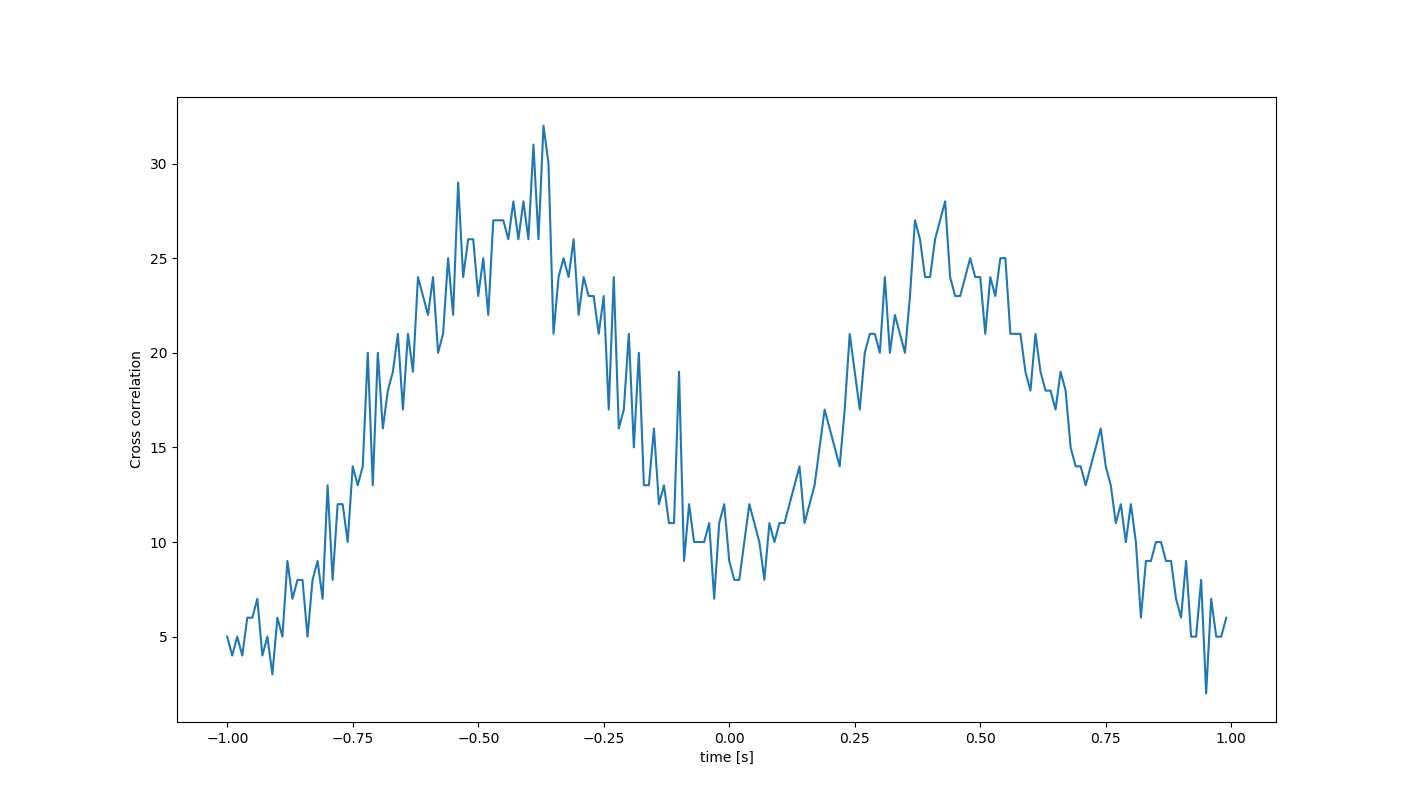
\includegraphics[scale=0.4]{1_a_pi.png}
\caption{Cross correlation function of $r_1$ and $r_2$ for $\omega = \pi$.}
\end{figure}

\begin{figure}[H]
\centering
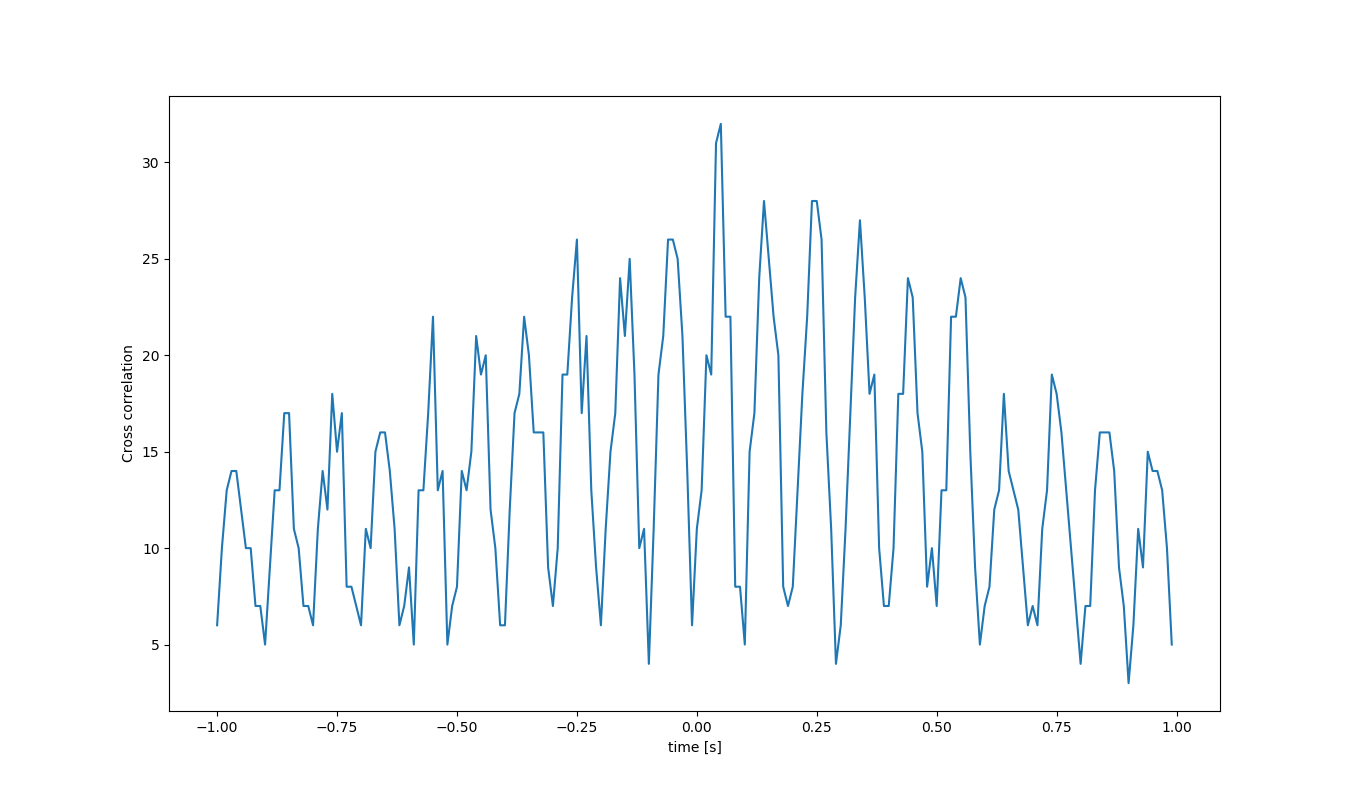
\includegraphics[scale=0.4]{1_a_10pi.png}
\caption{Cross correlation function of $r_1$ and $r_2$ for $\omega = 10\pi$.}
\end{figure}
\begin{figure}[H]
\centering
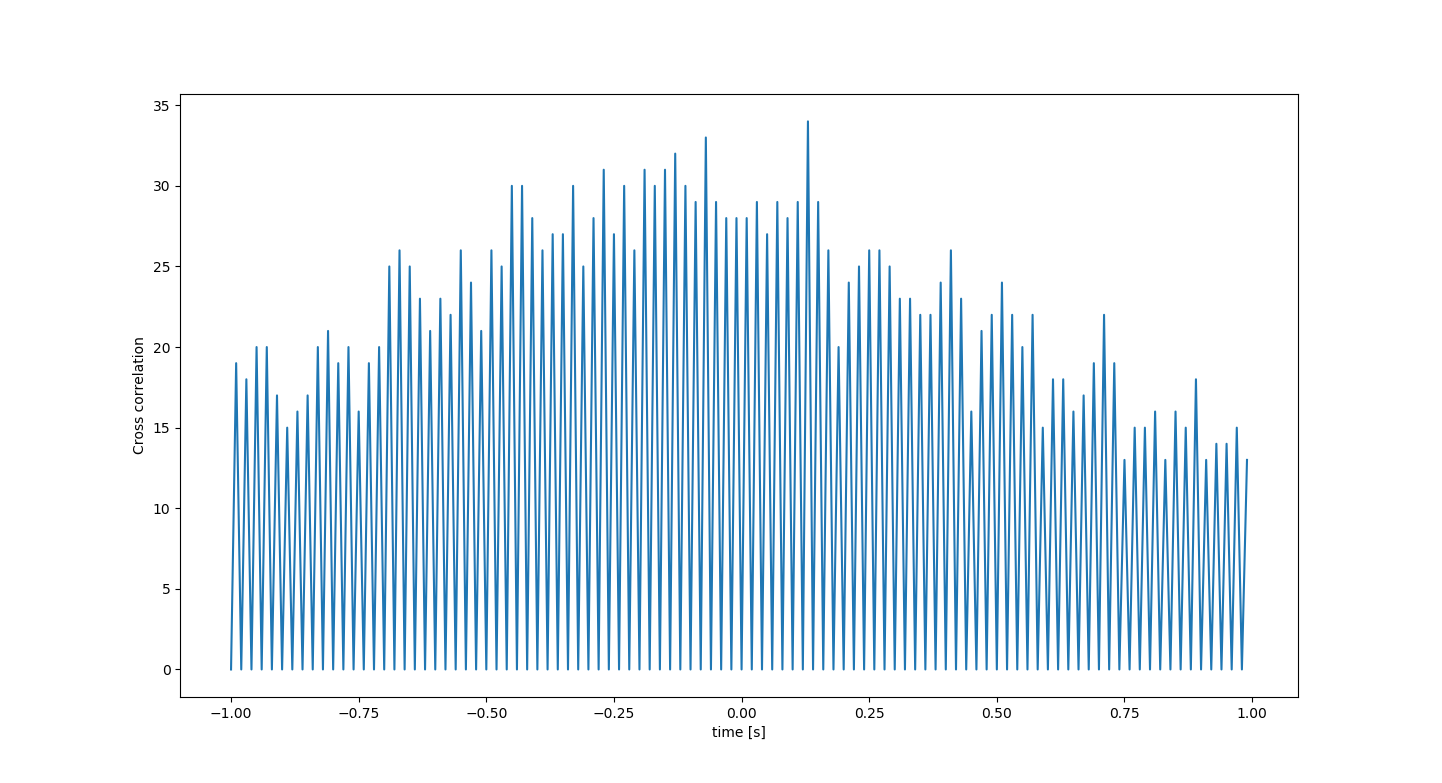
\includegraphics[scale=0.4]{1_a_50pi.png}
\caption{Cross correlation function of $r_1$ and $r_2$ for $\omega = 50\pi$.}
\end{figure}
Both, $sin(x)^2$ and $cos(x)^2$ are symmetric (with regards to $t = 0$) hence the cross correlation function has to be symmetric.\\
For $\omega >> r_0$ the frequency of the cross correlation function increases until it cannot be distinguished from $c(t) = 0$.
\newpage
\subsection*{b)}
Choosing $r_3(t) = r_0 * cos(\omega * (t - 0.3))^2$ (the function in a) has a peak at $0.5s$, so moving $r_2$ $0.3s$ to the right gives the desired result) gives a peak at $t = 200ms$:
\begin{figure}[H]
\centering
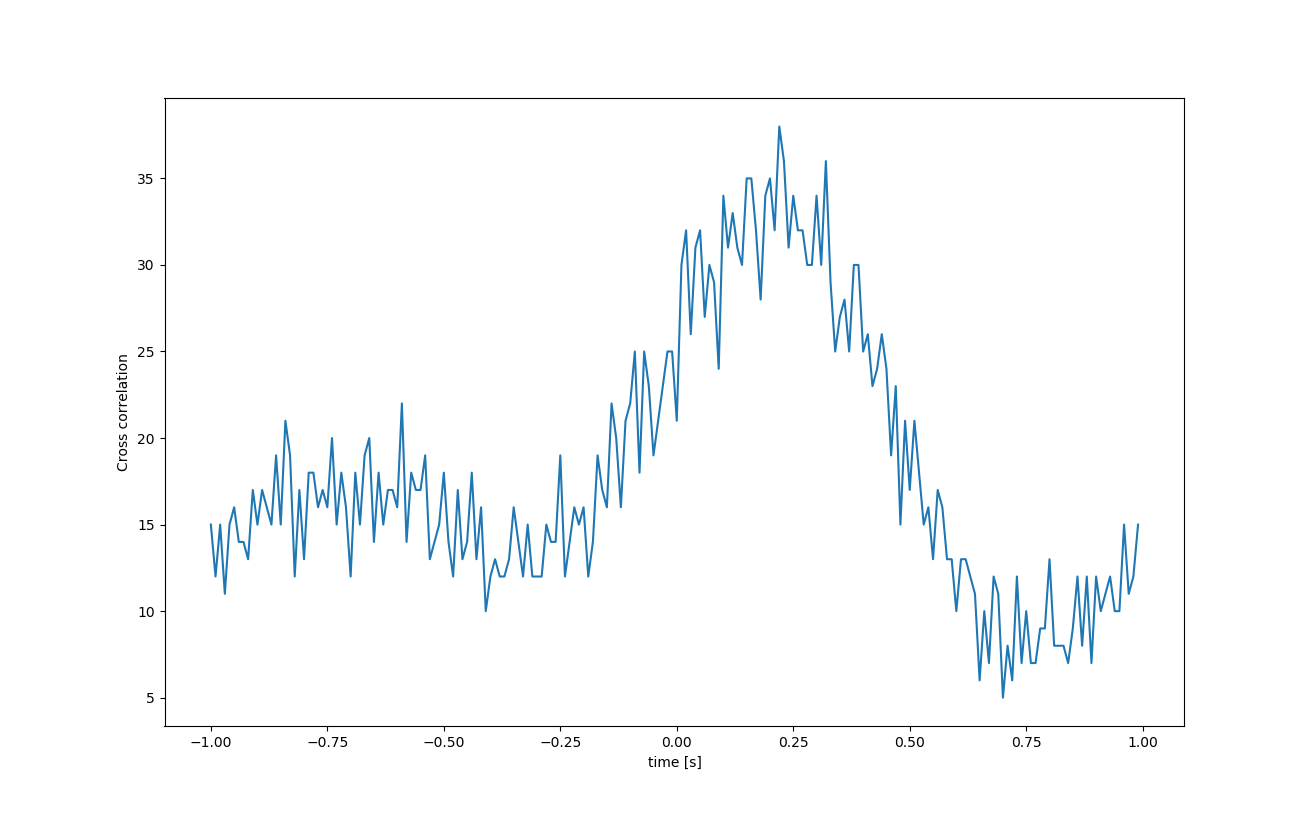
\includegraphics[scale=0.4]{1_b_pi.png}
\caption{Cross correlation function of $r_1$ and $r_3$ for $\omega = \pi$.}
\end{figure}

\newpage

\section*{2.}
\subsection*{a)}
\begin{figure}[H]
\centering
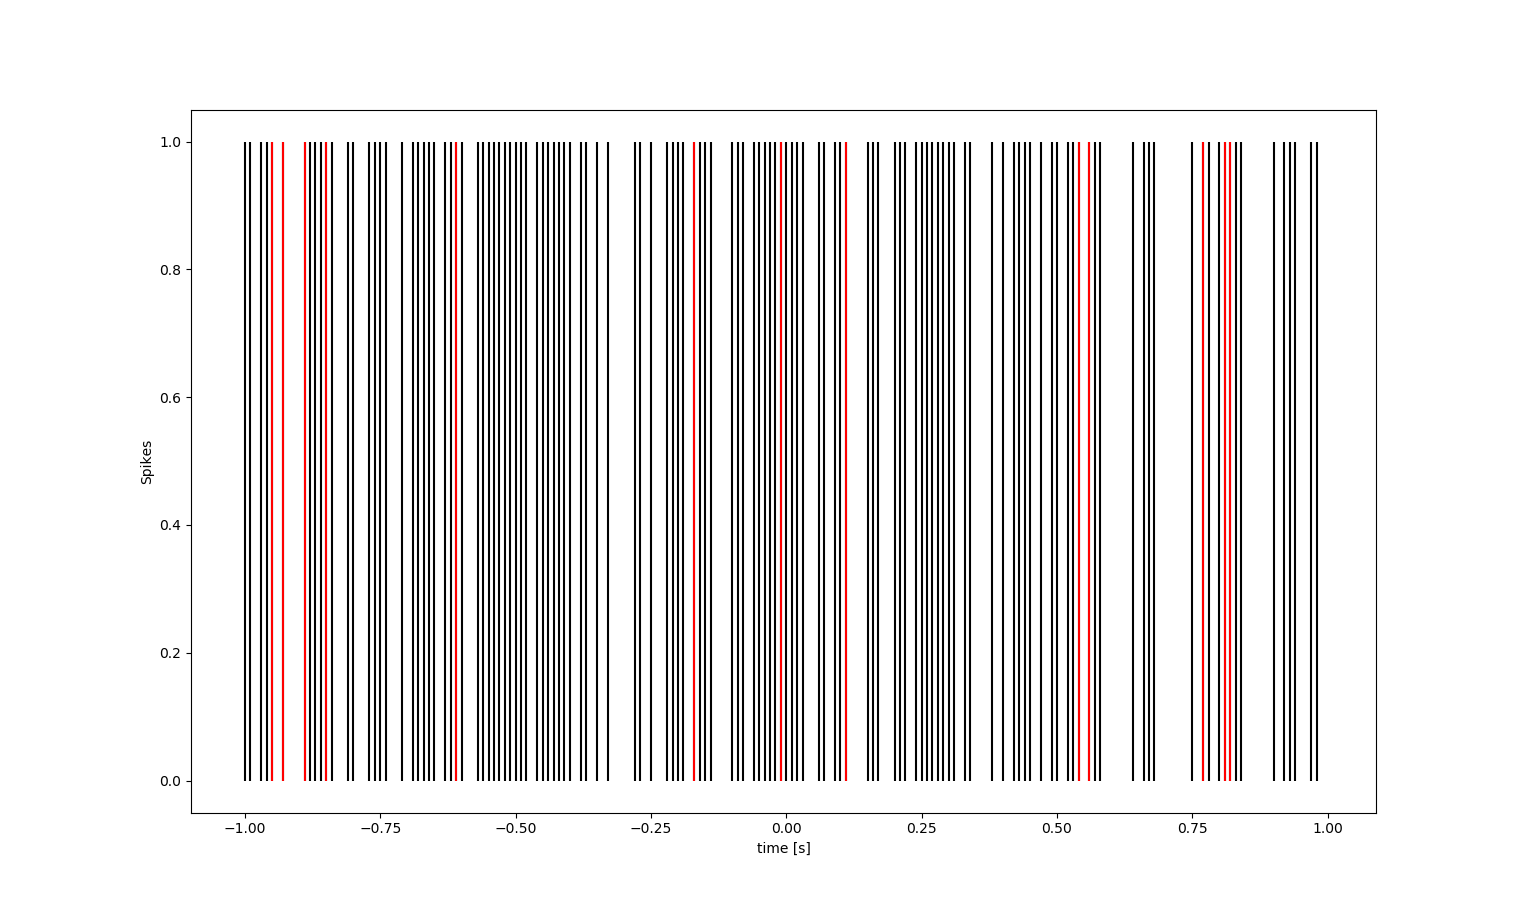
\includegraphics[scale=0.4]{2_c_p=0_1.png}
\caption{A parent train with frequency 60Hz (in black) and its child train (in red) with $p=0.1$.}
\end{figure}
The rate of the child train is given by $r_{parent} * p$.

\subsection*{b)}
\begin{figure}[H]
\centering
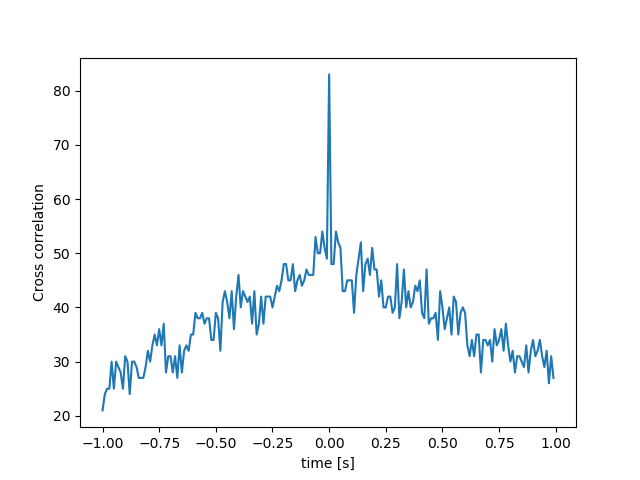
\includegraphics[scale=0.7]{2_b_p=0_7_0_0.png}
\caption{Cross correlation function with $p=0.7$ and no jitter.}
\end{figure}

\begin{figure}[H]
\centering
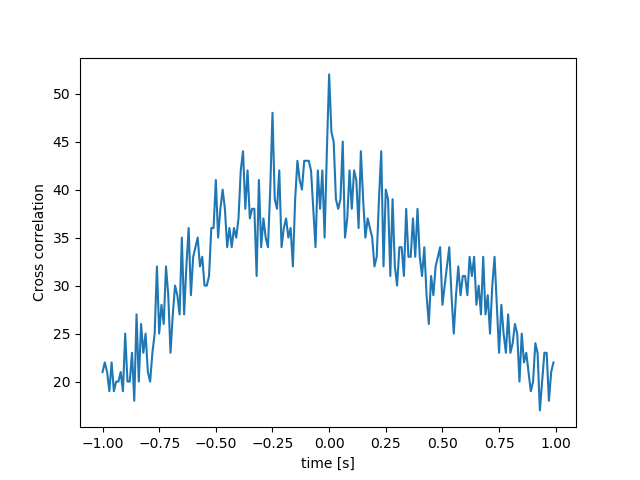
\includegraphics[scale=0.7]{2_b_p=0_7_2_0.png}
\caption{Cross correlation function with $p=0.7$ and $\sigma^2 = 0.02s, \mu = 0s$.}
\end{figure}

\begin{figure}[H]
\centering
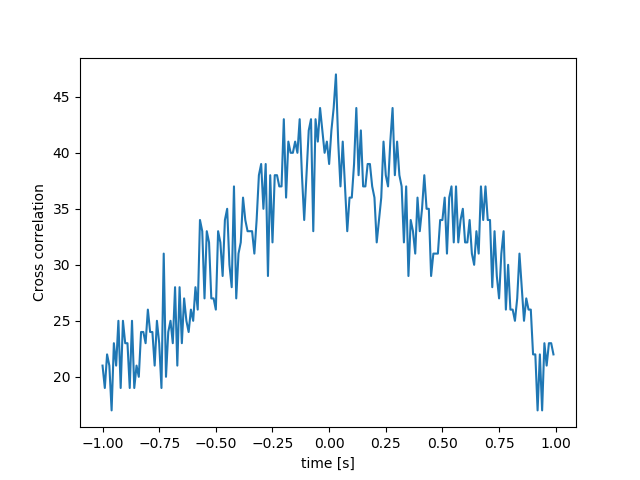
\includegraphics[scale=0.7]{2_b_p=0_7_50_0.png}
\caption{Cross correlation function with $p=0.7$ and $\sigma^2 = 0.5s, \mu = 0s$.}
\end{figure}

\begin{figure}[H]
\centering
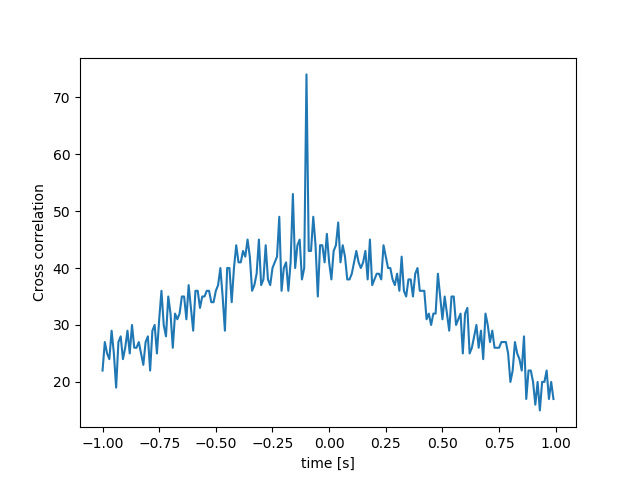
\includegraphics[scale=0.7]{2_b_p=0_7_0_10.png}
\caption{Cross correlation function with $p=0.7$ and $\sigma^2 = 0s, \mu = 0.10s$.}
\end{figure}

\begin{figure}[H]
\centering
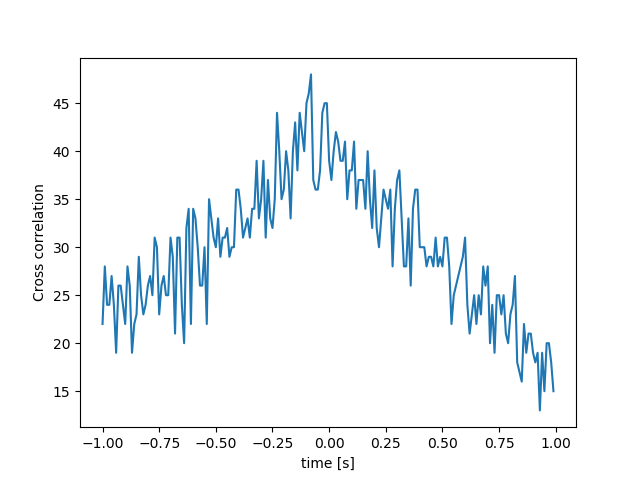
\includegraphics[scale=0.7]{2_b_p=0_7_2_10.png}
\caption{Cross correlation function with $p=0.7$ and $\sigma^2 = 0.02s, \mu = 0.10s$.}
\end{figure}

\subsection*{c)}
If we choose similar to the $\sigma^2 = 0s, \mu = 0.10s$ case in a) $\mu$ to be $-0.2s$ we can move the peak to the right:

\begin{figure}[H]
\centering
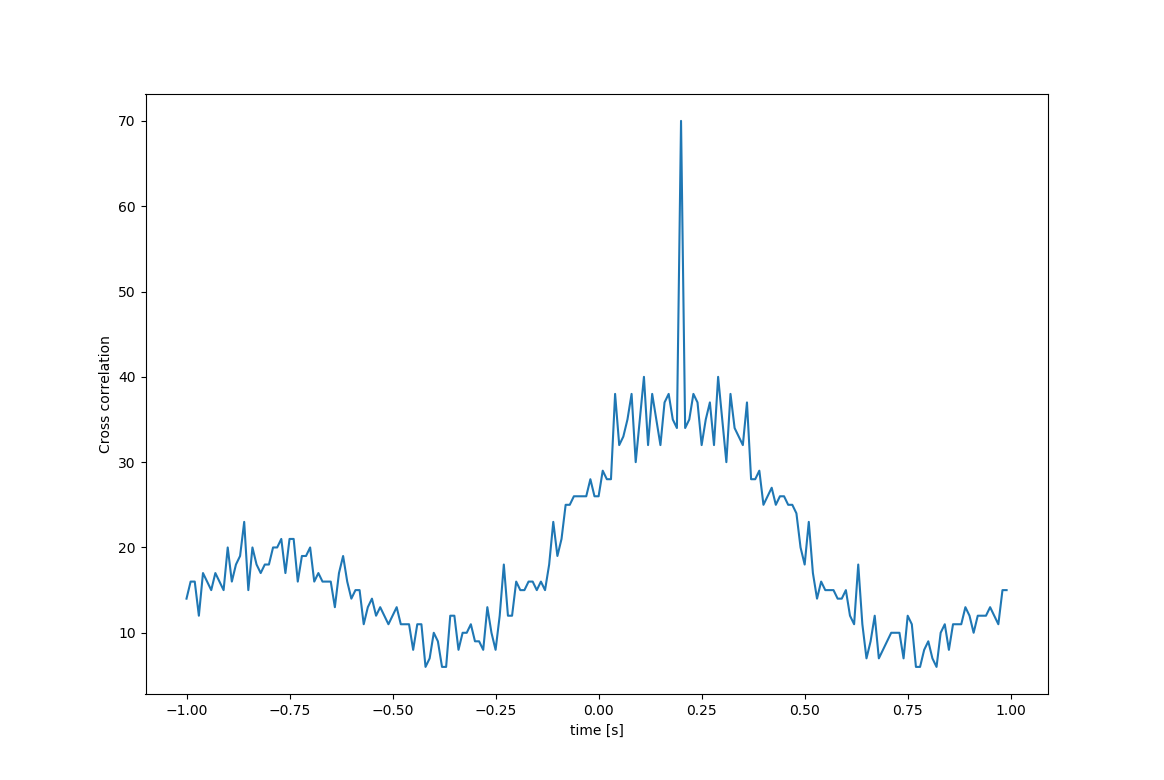
\includegraphics[scale=0.4]{2_c_p=0_5.png}
\caption{Cross correlation function of $r_1$ with $p=0.5$ and $\sigma^2 = 0s, \mu = -0.2s$.}
\end{figure}

\newpage
Increasing $\omega$ has the same effect as in 1c):
\begin{figure}[H]
\centering
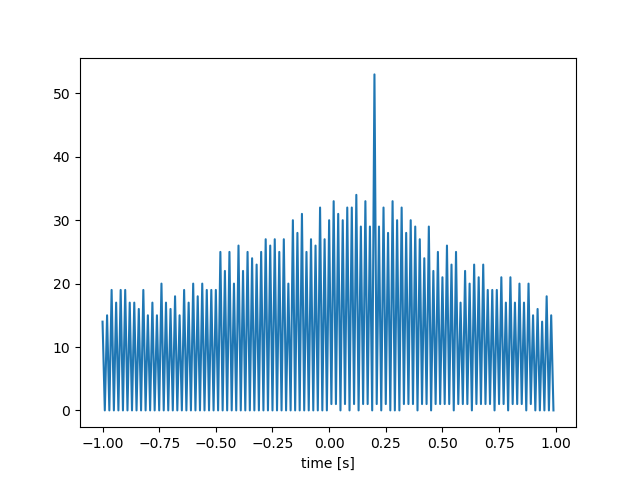
\includegraphics[scale=0.7]{2_c_p=0_5_omega=50pi.png}
\caption{Cross correlation function of $r_1$ with $p=0.5$, $\sigma^2 = 0s, \mu = -0.2s$ and $\omega=50\pi$.}
\end{figure}